\UseRawInputEncoding
\documentclass[11pt,letterpaper]{article}
\usepackage[margin=1.2in]{geometry}
\usepackage{amsmath, amssymb}
\usepackage{times}
\usepackage[mathscr]{euscript}
%\usepackage{mathrsfs}
\usepackage{graphicx}
\usepackage{color}
\usepackage[normalem]{ulem}
\usepackage{bm}
\usepackage{epstopdf}
\numberwithin{equation}{section}
\usepackage{mathrsfs}
\usepackage[round]{natbib}
\usepackage{subcaption}
\graphicspath{ {images/} }
 \usepackage[table]{xcolor}
\usepackage{longtable}
\usepackage[margin=1.2in]{geometry}
\usepackage{amsmath, amssymb}
\usepackage{amsthm}
\usepackage{times}
\usepackage[mathscr]{euscript}
%\usepackage{mathrsfs}
\usepackage{graphicx}
\usepackage{color}
\usepackage[normalem]{ulem}
\usepackage{bm}
\usepackage{epstopdf}
\numberwithin{equation}{section}
\usepackage{mathrsfs}
\usepackage[round]{natbib}
\usepackage{subcaption}
\graphicspath{ {images/} }
 \usepackage[table]{xcolor}
\usepackage{longtable}
\usepackage{array}
\usepackage{relsize}
\usepackage{pdflscape}
\usepackage[margin=1.2in]{geometry}
\usepackage{amsmath, amssymb}
\usepackage{times}
\usepackage[mathscr]{euscript}
%\usepackage{mathrsfs}
\usepackage{graphicx}
\usepackage{color}
\usepackage[normalem]{ulem}
\usepackage{bm}
\usepackage{epstopdf}
\numberwithin{equation}{section}
\usepackage{mathrsfs}
\usepackage[round]{natbib}
\usepackage{subcaption}
\graphicspath{ {images/} }
 \usepackage[table]{xcolor}
\usepackage{longtable}
\usepackage{array}
\newcolumntype{P}[1]{>{\centering\arraybackslash}p{#1}}
\usepackage{changepage}
\usepackage[affil-it]{authblk}
\usepackage{multirow, booktabs}
\usepackage{multicol}
\usepackage[nodisplayskipstretch]{setspace}
\usepackage{rotating}

\usepackage{bbm}

\newtheorem{theorem}{Theorem}[section]
\newtheorem{lemma}[theorem]{Lemma}

\newcommand{\xTilda}{\tilde{\bm{x}}}
\newcommand{\zZ}{Z^\star}
\newcommand{\zz}{z^\star}


\begin{document}
\title{Modeling  Frequency and Severity of Claims with the Generalized  Cluster-Weighted Model}

\author{Nikola Po\v cu\v ca, Tatjana Miljkovic,  Petar Jevti\' c and Paul D. McNicholas}

\maketitle
\doublespacing
\small

\begin{abstract}

In this paper, we propose a generalized cluster-weighted model (GCWM) that allows for modeling non-Gaussian distribution of the continuous covariates and a new zero-inflated GCWM (ZI-GCWM) for modeling insurance claims data with excess zeros. We describe two expectation-optimization (EM) algorithms for parameter estimation in GCWM and ZI-GCWM. A simulation study showed that both cluster models perform well for different settings in contrast to the existing mixture-based approaches. A real data set based on French automobile policies is used to illustrate the application of the proposed models.

\end{abstract}
\textsc{Key Words:} GCWM, CWM, ZI-GCWM, clustering, automobile claims.\\
\textsc{JEL Classification:}  C02, C40, C60.\\
% C02-Mathematical Methods, C40-General mathematical and statistical methods: special topics, c60-General mathematical methods, programming models, mathematical and simulation modeling%
\section{Introduction}\label{sec:introduction}
A significant number of clustering methods have been proposed for sub-grouping the data in the area of computer science, biology, social science, statistics, marketing, etc. \cite{Ingrassia+Punzo+Vittadini+Minotti:2015} proposed a cluster-weighted model (CWM) framework as a flexible family of mixture models for fitting the joint distribution of a random vector composed of a response variable and a set of mixed-type covariates with the assumption that continuous covariates come from Gaussian distribution. CWMs with Gaussian assumptions have been proposed by \cite{Gershenfeld:1997}, \cite{Gershenfeld:Schoner+Metois:1999}, and \cite{Gershenfeld:1999} in a context of media technology. Some extensions of this class of models have been considered by \cite{Punzo+Ingrassia:2015}, \cite{Ingrassia+Minotti+Punzo:2014}, \cite{Ingrassia+Minotti+Vittadini:2012}, \cite{subedi13,subedi15}, and \cite{punzo17}. These clustering methods are somewhat lacking for modelling insurance data, e.g., high excess zeros for claim count, heavy-tail loss distribution, deductible, or limits.

Sub-grouping of insurance policies based on risk classification is a standard practice in insurance. The heterogenous nature of insurance data allows for explorations of many different techniques for sub-grouping risk. As a result, there is a growing number of papers in the area of mixture modeling of univariate and multivariate insurance data to account for heterogeneity of risk. \cite{Lee+Lin:2010}, \cite{Verbelen+Gong+Antonio+Badescu+Lin:2015}, and \cite{Miljkovic+Grun:2016} proposed mixture models for univariate loss data, and mixture modeling of univariate insurance data has been extended to the multivariate context. A finite mixture of bivariate Poisson regression models with an application to insurance ratemaking was studied by \cite{Bermudez+Karlis:2012}. A Poisson mixture model for count data was considered by \cite{Brown+Buckley:2015} with application in managing a Group Life insurance portfolio. Recently, \cite{risks_miljkovic} reviewed two complementary mixture-based clustering approaches (CWMs and mixture-based clustering for an ordered stereotype model) for modeling unobserved heterogeneity in an automobile insurance portfolio, depending on the data structure under consideration. 

In this paper, we extend the CWM family proposed by \cite{Ingrassia+Punzo+Vittadini+Minotti:2015} to allow for modeling of non-Gaussian continuous covariates and a zero-inflated Poisson (ZIP) claims data with excess zeros, which are commonly seen in the insurance applications. We consider a generalized cluster-weighted model (GCWM) as well as a zero-inflated GCWM (ZI-GCWM). Two partitioning methods are considered with two separate expectation-maximization (EM) algorithms \citep{Dempster+Laird+Rubin:1977}. \textcolor{blue} {The EM algorithm is based on the complete-data likelihood, which encompasses the observed data together with the missing data and/or latent variables. The EM algorithm can be highly effective for maximum likelihood estimation when data is incomplete or is assumed to be incomplete.} The first EM algorithm is for parameter estimation for the GCWM models, while the second EM is for parameter estimation for the ZI-GCWM. We show that the Bernoulli and Poisson GCWM accurately estimate the initialization of the EM algorithm for the ZI-GCWM model. These models utilize individual claims data and should be useful in the areas of ratemaking and risk management.

This paper is organized as follows. The GCWM and GCWM approaches are discussed in Section~\ref{sec:model}, and parameter estimation is discussed in Section~\ref{sec:estmeth}. Then, our methodology is applied to real data on French automobile claims and an extensive simulation study is conducted (Section~\ref{sec:numapp}). This paper concludes with a discussion and some suggestions for future work (Section~\ref{sec:sim}).


\section{Methodology}\label{sec:model}

\subsection{Background}

Let $(\bm{X^{'}}, Y)^{'}$  be the pair of a vector of covariates  $\bm{X}$ and a response variable $Y$. Assume this pair is defined on some sample space $\Omega$ that takes values in an appropriate Euclidian subspace. Now, assume that there exists $G$ non-overlapping partitions of $\Omega$, denoted as $\Omega_1, \ldots, \Omega_G$.  \cite{Gershenfeld:1997} characterized CWMs as a finite mixture of GLMs; hence, the joint distribution $(\bm{X^{'}}, Y )^{'}$ has the form
 \begin{align}
 f(\bm x, y; \bm{\Phi})= \sum_{j=1}^{G} \tau_j q(y|\bm{x};\bm{\vartheta}_j)p(\bm{x};\bm{\vartheta}_j),
\label{eq1}
\end{align}
where $\bm{\Phi}$ denotes the model parameters.
%
The pair $q(y|\bm{x};\bm{\vartheta}_j)$ and $p(\bm{x};\bm{\vartheta}_j)$ are conditional and marginal distributions of $(\bm{X^{'}}, Y)^{'}$, respectively, while $\tau_j$ is the $j$th mixing proportion such that $\sum_{j=1}^{G}\tau_j=1$, $\tau_j>0$.
\cite{Ingrassia+Punzo+Vittadini+Minotti:2015} proposed a flexible family of mixture models for fitting the joint distribution of a random vector $(\bm{X^{'}}, Y)^{'}$ by splitting the covariates into continuous and discrete, i.e., $ \bm{X}=(\bm{V}',  \bm{W}')'$. The assumption of independence between continuous and discrete covariates allows us to multiply their corresponding marginal distributions. Thus, for this setting the model in \eqref{eq1} is reformulated as follows
\begin{align}
 f(\bm{x}, y; \bm{\Phi})= \sum_{j=1}^{G} \tau_j q(y|\bm{x};\bm{\vartheta}_j)p(\bm{x};\bm{\theta}_j)=\sum_{j=1}^{G} \tau_j q(y|\bm{x};\bm{\vartheta}_j)p(\bm{v}; \bm{\theta}_j^{\star})p(\bm{w};\bm{\theta}_j^{\star\star})
\label{eq2}
\end{align}
where $\bm{v}$ and $\bm{w}$ are the vectors of continuous and discrete covariates, respectively, $q(y|\bm{x};\bm{\vartheta}_j)$ is the conditional density of $Y|\bm{x}$ with parameter vector $\bm{\vartheta}_j$, $p(\bm{v};\bm{\theta}_j^{\star})$ is the marginal distribution of $\bm{v}$ with parameter vector $\bm{\theta}_j^{\star}$, and $p(\bm{w};\bm{\theta}_j^{\star\star})$ is the marginal distribution of $\bm{w}$ with parameter vector $\bm{\theta}_j^{\star\star}$. As before, $\bm{\Phi}$ denotes the model parameters. %Nik: this does not seem to be all model parameters? Also, vartheta is either bold face (vector) or not (scalar), and what is $\lm$?. % Notation Corrected - Nik
Note that the conditional distribution $q(y|\bm{x};\bm{\vartheta}_j)$ is assumed to belong to an exponential family of distributions and as such can be modeled in the GLM framework. Here, the marginal distribution of continuous covariates is assumed to be Gaussian. Unfortunately, this last assumption is too strong for use in insurance related applications, specifically in rate-making. To relax it, we develop the GCWM, which allows for non-Gaussian covariates as discussed in the next section.

\subsection{Generalized cluster-weighted model (GCWM) }
We proceed to extend \eqref{eq2} by splitting the continuous covariates $\bm{V}$ via $\bm{V}=(\bm U^{'}, \bm T^{'})^{'}$, where $\bm{U}$ contains the non-Gaussian covariates and $\bm{T}$ contains the Gaussian covariates. Thus \eqref{eq2} becomes
\begin{align}
 f(\bm x, y; \bm{\Phi})= \sum_{j=1}^{G} \tau_j q(y|\bm{x};\bm{\vartheta}_j)p(\bm{t};\bm{\theta}_j^{\star})p(\bm{w};\bm{\theta}_j^{\star\star})p(\bm{u};\bm{\theta}_j^{\star\star\star}),
\label{eq3}
\end{align}
which we refer to as the GCWM. Here, $p(\bm{t};\bm{\theta}_j^{\star})$ denotes the marginal density of Gaussian covariates, with parameter vector $\bm{\theta}^{\star}$, and $p(\bm{u};\bm{\theta}_j^{\star\star\star})$ is the marginal density of the non-Gaussian covariates with parameter vector $ \bm{ \theta}_j^{\star\star\star} $.


Because of its relevance to the actuarial application in this paper, we focus on the multivariate log-normal distribution  for non-Gaussian covariates --- this, however, does not reduce the generality of our general framework. With the log-normal assumption for $p(\bm{u};\bm{\theta}_j^{\star\star\star})$, we have that $\bm{u}$ is defined on $\mathbb{R}^p_+$ with parameter vector $\bm{\theta}_j^{\star\star\star}= (\bm{\mu}_j^{\star\star\star} ,\bm{\Sigma}_j^{\star\star\star})$ and probability density function
\begin{equation}\label{eqn:logn} 
p \left(  \bm{u}; \bm{\theta}_j^{\star\star\star} \right) = \frac{1}{(\prod_{i=1}^{p}u_{i})|\bm{ \Sigma}_j^{\star\star\star} |(2 \pi)^{\frac{p}{2}}}   \exp\left[-\frac{1}{2}(\ln\bm{ u}-\bm{\mu}_j^{\star\star\star})^{'}\bm{\Sigma}_j^{{\star\star\star}_{-1}}(\ln \bm {u}-\bm{\mu}_j^{\star\star\star})\right].
\end{equation} The derivation of \eqref{eqn:logn} can be found in the Appendix \ref{changeVarUni}.

%Nik: is this a density? What range of values of x? What values can mu and sigma take?
% PM: Is this more clear?

\subsection{Zero-inflated Poisson Model}%Nik: not sure what this means? Specifically, what is the role of the first "-"

In the zero-inflated Poisson (ZIP) model \citep[see][]{Lambert}, we can split the conditional density of the response variable $Y$, i.e., $p(y|\bm{x},\bm{\vartheta}_j)$, into zero and non-zero densities. The conditional probability mass associated with the event $y=0$ is characterized by $q(y = 0|\bm{x},\bm{\vartheta}_{j})$. For situations when $y > 0$, the response variable $Y$ is conditionally distributed with density $q(y > 0|\bm{x}, \bm{\vartheta}_{j} )$. Given the conditional density for the ZIP model, \eqref{eq3} can be re-written as
 \begin{align}
 f(\bm x, y; \Phi)= \sum_{j=1}^{G} \tau_j \left[ q(y = 0|\bm{x};\bm{\vartheta}_{j} ) +  q(y > 0|\bm{x} ; \bm{\vartheta}_{j}  ) \right]   p(\bm{t};\bm{\theta}_j^{\star})p(\bm{w};\bm{\theta}_j^{\star\star})p(\bm{u};\bm{\theta}_j^{\star\star\star}).
\end{align}

Define $\xTilda = [\bm{1},\bm{x}]$, which contains the covariates together with a placeholder for the intercept in the GLM. Denote the Poisson conditional density  as $ q^P(y|\bm{x}; \lambda_j) $, where $y \in \{0,1,\dots\}$, and let $\bm{\beta}_j$ be a row coefficient vector.
The link function will be modelled with log-link for the GLM such that
 \begin{align*}
\lambda_j = e^{\xTilda \bm{\beta}_j'} && \text{and} & & %\beta_{0j} + \beta_j^{'}x
q^P(y|\bm{ x} ; \lambda_{j} ) = e^{-\lambda_j} \frac{{\lambda_j}^y}{y!}.
 \end{align*}
Now, we use a Bernoulli model for the conditional density. We denote the density as $ q^{B}(y|\bm{x}; \bm{\bar{\beta}}_j) $, where $\bar{\bm{\beta}_j}$ is a row coefficient vector.  Here, the GLM will be modelled with the associated logit link function so that
 \begin{align*}
 \psi_j =  \frac{e^{\xTilda \bm{\bar{\beta}}_j'}}{1+ e^{\xTilda  \bm{\bar{\beta}}_j'}}  && \text{and} && 
 q^B(y | \bm{x} ; {\psi}_j) = \begin{cases}
      \quad \psi_j, & y = 0,\\
     1 -  \psi_j,  & y > 0.
   \end{cases}
 \end{align*}
 Now, given a combination of two preceding models, we introduce the ZIP model in which zero counts come from two random variables. One is the Bernoulli random variable, which generates structural zeros, and the other is the Poisson random variable. The coefficients $\bm{\vartheta}_{j}=\{ \bm{\beta}_{j},  \bm{\bar{\beta}}_j \}$ correspond to the two above introduced conditional densities where the coefficients are estimated using a GLM as in \cite{Lambert}. The components of ZIP conditional density $q(y|\bm{x}; \bm{\vartheta}_{j}  )$ are %Nik: something missing here?, PM: Fixed.
 \begin{align*}
 q( y = 0| \bm{x} ; \bm{ \vartheta}_{j}  ) = \psi_j + (1 - \psi_j)e^{-\lambda_j}  & &  \text{and}  & &
q(y > 0 |  \bm{x} ; \bm{ \vartheta}_{j}  ) = (1 - \psi_j)e^{-\lambda_j} \frac{\left(\lambda_j \right)^y  }{y!}.
 \end{align*}
Also, the link functions we consider are log-link for the Poisson and logit link for the Bernoulli model so that
 \begin{align}
 \psi_j =  \frac{e^{\xTilda \bm{\bar{\beta}}_j'}}{1+ e^{\xTilda \bm{\bar{\beta}}_j'}}  & & \text{and} & &
\lambda_j  = e^{\xTilda \bm{\beta}_j'}. \label{bern::ref}
 \end{align}
Noe that, here, the parameter $\psi_j$ denotes the mean of the Bernoulli distribution of the $j$th component from which extra zeros emanate, and the parameter $ \lambda_j $ characterizes the $j$th Poisson distribution. This allows for a more nuanced approach to handling the inflation of zeros for automobile insurance  \citep[see][]{Bermudez+Karlis:2012}.

\subsection{Bernoulli-Poisson Sample Space Partitioning}

The single component ZIP model assumes that the inflated zeros emanate from both a Bernoulli and Poisson random variables while the non-zeros are assumed to come exclusively from the Poisson random variable. However, recent research  extends the single component ZIP models to mixture models for heterogeneous count data with excess zeros \citep[see][]{Bermudez+Karlis:2012}. In mixtures of ZIPs, zeros are assumed to come from multiple different Binomial and Poisson random variables. Difficulties are apparent  during the maximization step of the EM algorithm when means of covariates are very close together \cite[see][]{LimHwa}. However, misclassification error can be reduced using parsimonious models for the independent variables as in  \cite{McNicholas:2010}. \textcolor{red}{[Is this the paper we mean to cite?]} \textcolor{blue}{In your paper with  TB Murphy found here: https://pdfs.semanticscholar.org/6e54/f621ff1c43c3bac0ba989953e7253b5fa4c0.pdf
}
	In this work, we propose a new method to rectify this problem and partition the dataset using Bernoulli and Poisson GCWMs. Furthermore, we construct a ZI-GCWM using the previously generated Bernoulli and Poisson GCWMs. By using the EM algorithm, we estimate parameters pertaining to the GCWM under the assumption of a Poisson model and, separately, we carry out the same process under the assumption of a Bernoulli model. Using the obtained parameter estimates from the two separate applications of the EM algorithm, we set the initialization parameters for the EM algorithm for parameter estimation for the ZI-GCWM. The work of \cite{Lambert} specifies that the MLE estimates for the separate Poisson and Bernoulli models provide an excellent initial guess, allowing EM to converge quickly for ZIPs. The Bernoulli-Poisson sample space partitioning method consists of two separate EM algorithms. The first EM algorithm is for generating the GCWM models, while the second EM is for optimizing the ZI-GCWM. Recall $(\bm {X^{'}}, Y)^{'}$ to be a vector defined on some sample space $\Omega$.  Also by assumption, this sample space is partitioned into $K$ non-overlapping sets such that their union constitutes it ie. $ \Omega = \bigcup_{i=1}^K \Omega_i $. \textcolor{red}{[I do not think this has been discussed. I am not sure it is helpful?]}  \textcolor{red}{[In what precise sense does a set have a shape?]} 
\textcolor{blue}{
For each particular set $\Omega_i$, a pure Poisson or a zero-inflated Poisson model may exist. For partitions relating to the zero-inflated Poisson model,  the choice on the $ith$ group will further partition $\Omega_i$ such that $\Omega_i = \Omega^{B}_i \cap \Omega^{P}_i  $, where $\Omega^{B}_i$ is the sample space of excess zeros emanating from a Bernoulli model, $\Omega^{P}_i$ is the sample space relating to a Poisson model. This allows for the construction of both pure Poisson, and zero-inflated Poisson mixtures to exist on $\Omega$.   }
	 \textcolor{red}{[I am not sure that all the material about sample spaces in the following is helpful here. Thoughts?]} Specifically, if we introduce the Bernoulli model in a generalized form for conditional density \citep[see][for specific cases]{Ingrassia+Punzo+Vittadini+Minotti:2015}, we have the sample space $\Omega^B$ and joint probability density function $f^B$ to be \begin{align*}
\Omega^B =  \bigcup_{l =1}^{M \leq G}  \Omega_l^B & & \text{and} &  &
f^B(\bm x, y; \Phi)= \sum_{l=1}^{M \leq G} \tau_l q^B(y|\bm{x}; \bm{\bar{\beta}}_l) p(\bm{t};\bm{\theta}_l^{\star})p(\bm{w};\bm{\theta}_l^{\star\star})p(\bm{u};\bm{\theta}_l^{\star\star\star}).
\end{align*}
Similarly, if we introduce a Poisson model in a generalized form the sample space $\Omega^P$ and joint probability density function $f^P$ become
\begin{align*}
\Omega^P =  \bigcup_{j =1}^G \Omega_j^P & & \text{and} &  &
f^P(\bm x, y; \Phi)= \sum_{j=1}^{G} \tau_j q^P(y|\bm{x};\bm{\beta}_{j}) p(\bm{t};\bm{\theta}_j^{\star})p(\bm{w};\bm{\theta}_j^{\star\star})p(\bm{u};\bm{\theta}_j^{\star\star\star}).
\end{align*}
Where this sample space is partitioned up to $M$ non-overlapping sets.
 Now, construct a new partitioning of a sample space $\Omega$ such that
$$\Omega = \left(\bigcup^G_{j=1} \Omega^P_j \right) \bigcup \left( \bigcup^{M \leq G}_{l=1} \Omega^B_l  \right) = \left( \bigcup_{k=1}^{M \leq G}  \Omega^P_k \cap \Omega^B_k \right) \bigcup \left( \bigcup_{j > M}^G \Omega^P_j \right) $$ 
$$:= \left(  \bigcup_{k=1}^{M \leq G} \Omega_k^Z \right) ]\bigcup \left( \bigcup_{j > M}^G \Omega^P_j \right)  $$
where $\Omega^Z_k$ is the $k$th partition related to the zero-inflated Poisson model, and $\Omega^P_j$ is the  $j$th partition related to the pure Poisson model.   Therefore the new conditional density for $\Omega^Z_k$ is now result of a model in which each component is captured by the conditional probability density function that is a mixture of particular Bernoulli and particular Poisson densities
\begin{align}
q^Z_{k}(y|\bm{x};  \bm{\bar{\beta}}_k,\bm{ \beta}_k) & := q^B(y|\bm{x}; \bm{\bar{\beta}}_k) +(1-  q^B(y|\bm{x}; \bm{\bar{\beta}}_k) ) q^P(y|\bm{x};\bm{\beta}_k) \nonumber \\
& = q(y = 0|\bm{x};\bm{\vartheta}_{k} ) +  q(y > 0|\bm{x} ; \bm{\vartheta}_{k}), \quad k \in \{1 ,\ldots, K \}.
\label{ziGCWM}
\end{align}

The initialization parameters for the second EM algorithm are provided by Bernoulli and Poisson GCWMs from \eqref{ziGCWM} giving parameter pairs ($ \psi_k,\lambda_k  $). The second EM procedure then optimizes \eqref{ziGCWM}. The ZI-GCWM is then compared against the standard Poisson GCWM using a likelihood ratio test which is discussed in Section~\ref{subsec:: compareZero}.

\section{Parameter Estimation}\label{sec:estmeth}

The common approach for estimating parameters in finite mixture models is based on the EM algorithm \citep[see][for examples]{mcnicholas16a}.
The estimation of the developed Bernoulli-Poisson partitioning method is split into two EM algorithms. The first EM algorithm partitions the sample space, while the second EM algorithm optimizes the zero inflated portion.
 %Nik: this is incorrect. The EM algorithm does not estimate the optimal number of components.  PM: Removed.

\subsection{EM Algorithm for Partitioning of Sample Space}

The EM algorithm is based on the local  maximum likelihood estimation. %Nik: need to be careful here. Please reword. , PM: Local maximum?
The initial values of the parameter estimates can be generated from a variety of strategies outlined in \cite{initialPaperGrassiaRef}. %Nik: this may or may not be the case.
% PM: I cited the same paper ingrassia used for initializations.
 The algorithm proceeds by alternation of the E- and M-steps to update parameter estimates. %Nik: again, need to be much more careful.
%
The convergence criterion of the EM algorithm is based on the Aitken acceleration. It is used to estimate the asymptotic maximum of the log-likelihood at each iteration of the EM algorithm when the relative increase in the log-likelihood function is no bigger than a small pre-specified tolerance value or the number of iterations reach a limit. %Nik: that is a possible stopping rule but is not a convergence criterion per se.
To find an optimal number of components, maximum likelihood estimation is obtained over a range of $G$ groups, and the best model is selected based on the Bayesian information criterion (BIC).   %Nik: which one? Explain. %PM: BIC was used.

In this subsection, we explain the parameter estimation in line with the GCWM methodology proposed by \cite{Ingrassia+Punzo+Vittadini+Minotti:2015}. The proposed GCWM  is based on the assumption that $q(y|\bm{x},\bm{\vartheta}_j)$ belongs to the exponential family of distributions that are strictly related to GLMs. The link function defines the relationship between the linear predictor and the expected value of the distribution function as $g(\bm{\mu}_j)= \xTilda \bm{\beta}^{'}$, where $g(\bm{\mu}_j)$ is the link function. We are interested in the estimation of the vector $\bm {\beta}_j$, thus the distribution of $Y|\bm{x}$ is denoted by $q(y|\bm{x}; \bm{\beta}_j, \lambda_j)$, where $\lambda_j$ signifies an additional parameter to account for when a distribution belongs to a two-parameter exponential family.

The marginal distribution $p(\bm{x}; \bm \theta_j)$ has the following components: $p(\bm{t}; \bm \theta_j^{\star})$, $p(\bm{w}; \bm \theta_j^{\star\star})$, and $p(\bm{u};\bm \theta_{j}^{\star\star\star})$. The first marginal density \textcolor{blue}{ $p(\bm{t}; \bm \theta_j^{\star}:=( \bm {\mu}_j^{\star}, \bm{\Sigma}_j^{\star}) )$} is modeled as a  Gaussian distribution with mean $\bm {\mu}_j^{\star}$ and covariance matrix $\bm{\Sigma}_j^{\star}$. 
 The marginal density of discrete covaraites $p(\bm{w};\bm{\theta}_{j}^{\star\star})$ is assumed to have for each finite discrete covariate in $\bm{W}$, a representative binary vector $\bm{w}^r=(w^{r1},\ldots,w^{rc_r})^{'}$, where $w^{rs}=1$ if $w_r = s\in\{1, \ldots, c_r\}$, %Nik: this wording seems very awkward. Does "has the value" just mean "="? If so, why not write "="?
and $w^{rs}=0$ otherwise.
\textcolor{red}{[As mentioned before, the following equation seems to come out of nowhere.]}
\textcolor{blue}{Given the preceding assumptions about discrete covariates, the marginal density is written as}
\begin{align}
p(\bm {w}; \bm {\gamma_j})=\prod_{r=1}^{d}\prod_{s=1}^{c_r}(\gamma_{jrs} )^{w^{rs}}
\label{eq31}
\end{align}
for $j=1, \ldots, G$, where $\bm {\gamma}_j=(\gamma_{j1}^{'}, \ldots, \gamma_{jd}^{'})^{'}$, $\bm \gamma_{jr}=(\gamma_{jr1}^{'}, \ldots, \gamma_{jrc_d}^{'})^{'}$, $\gamma_{jrs} > 0$, and  $\sum_{s=1}^{c_r}\gamma_{jrs}$, $r=1,\ldots,q$. The density $p(\bm {w}, \bm{\gamma}_j)$ represents the product of $d$ conditionally independent multinomial distributions with parameters $\bm{\gamma}_{jr}$, $r=1,\ldots, d$. Finally, the third marginal density $p(\bm{u};\bm{\theta}_{j}^{\star\star\star})$ will be modelled with a multivariate log-normal distribution having a location parameter vector $ \bm{\mu}_j^{\star\star\star}$ and scale parameter matrix $\bm{\Sigma}_j^{\star\star\star} $.

Let $(\bm x_1, y_1),\ldots, (\bm x_n, y_n)$ be a sample of $n$ independent observations drawn from model in \eqref{eq3}. Consider a latent random variable $Z_{ij}$.  The realization $z_{ij}$ of the latent indicator variable takes the value of $z_{ij}=1$ indicating that observation $(\bm{x_i}, y_i)$ originated from the $j$th mixture component and $z_{ij}=0$ otherwise.
 \textcolor{red}{[Need to explain complete-data earlier.]}  \textcolor{blue}{[I now understand, you meant introduce it in writing, not in definition]}

 Given the sample, the complete-data likelihood function $L_c(\bm\Phi)$ is given by
\begin{align}
L_c(\bm\Phi)=\prod_{i=1}^{n}\prod_{j=1}^{G}\left[{\tau_j}q(y_i|x_i; \bm \beta_j, \lambda_{j})p(t_i; \bm\mu_j^{\star}, \bm\Sigma_j^{\star}) p(w_i; \gamma_j)p(u_i; \bm{\mu}_j^{\star\star\star},\bm{\Sigma}_j^{\star\star\star}) \right]^{z_{ij}},
\label{eq27}
\end{align}

%
Taking the logarithm of \eqref{eq27}, the complete-data log-likelihood is 
\begin{equation}\begin{split}
\ell_c(\bm\Phi)= \sum_{i=1}^{n}\sum_{j=1}^{G}{z_{ij}}\big[\log(\tau_{j}) + \log{q}(y_i|x_i; \bm{\beta}_j,\lambda_j)+& \\ \log p(t_i; \bm{\mu}_j^{\star}, \bm{\Sigma}_j^{\star}) & + \log p(w_i; \bm{\gamma}_j) +\log {p}(u_i; \bm{\mu}_j^{\star\star\star},\bm{\Sigma}_j^{\star\star\star}) \big].
\label{CompleteLiklihood}
\end{split}\end{equation}

%\subsubsection{E-Step - Partitioning}
On the $(s+1)$th iteration, the E-step requires calculation of the conditional expectation of $\ell_c(\bm\Phi)$. Because $\ell_c(\bm\Phi)$ is linear with respect to  $z_{ij}$, we simplify the calculation to the current expectation of $Z_{ij}$, where $Z_{ij}$ is the random variable corresponding to the realization $z_{ij}$. Given the previous parameters $\bm\Phi^{(s)}$ and the observed data,  we calculate the current conditional expectation of $Z_{ij}$ as
\begin{equation*}\begin{split}
    {\pi_{ij}}^{(s)} &= {E}[Z_{ij} |(\bm{x_i}, y_i); \bm{\Phi}^{(s)}]\\
     &= \frac{{\tau_j}^{(s)}q(y_i|x_i; \bm \beta_j^{(s)}, \lambda^{(s)}_{j})p(t_i; \bm\mu_j^{{\star}(s)}, \bm\Sigma_j^{{\star}(s)}) p(w_i; \bm \gamma_j^{(s)})p(u_i; \bm{\mu}_j^{\star\star\star (s)},\bm{\Sigma}_j^{\star\star\star (s)})}{f(\bm{x}_i, y_i; \bm{\Phi}^{(s)})
\label{eq29}                       }.
\end{split}\end{equation*}
%
%\subsubsection{M-Step - Partitioning}
\textcolor{blue}{On the M-step of the $(s+1)$th iteration, the conditional expectation of $\ell_c(\bm\Phi)$ denoted as a function $Q(\Phi|\Phi^{(s)})$ is maximized with respect to $\Phi $ where}  \textcolor{red}{[What does the previous sentence mean? It seems to me that $Q(\Phi|\Phi^{(s)})$ is simply what is calculated on the E-step; however, what is written here suggests something quite different.]} the values of $z_{ij}$ in \eqref{CompleteLiklihood} are replaced by their current expectations $\pi_{ij}$ yielding 
\begin{equation}\begin{split}
Q(\bm\Phi|\bm\Phi^{(s)}) &= \sum_{i=1}^{n}\sum_{j=1}^{G}{\pi_{ij}^{(s)}} \big[\log(\tau_{j}) + \log{q}(y_i|x_i;\bm{\beta}_j,\lambda_j)+ \log p(t_i; \bm{\mu}_j^{\star}, \bm{\Sigma}_j^{\star})  + \log p(w_i; \bm{\gamma}_j)\\ 
&\qquad\qquad\qquad\qquad+\log {p}(u_i; \bm{\mu}_j^{\star\star\star },\bm{\Sigma}_j^{\star\star\star })\big] \\
&=\sum_{i=1}^{n}\sum_{j=1}^{G}{\pi_{ij}^{(s)} \log(\tau_{j}) + \sum_{i=1}^{n}\sum_{j=1}^{G}{\pi_{ij}^{(s)}}\log{q}(y_i|x_i;\bm{\beta}_j},\lambda_j) +\sum_{i=1}^{n}\sum_{j=1}^{G} {\pi_{ij}^{(s)}}\log p(t_i; \bm{\mu}_j^{\star}, \bm{\Sigma}_j) \\
&\qquad\qquad\qquad\qquad+\sum_{i=1}^{n}\sum_{j=1}^{G}{\pi_{ij}^{(s)}}\log p(w_i; \bm{\gamma}_j) + \sum_{i=1}^{n}\sum_{j=1}^{G}{\pi_{ij}^{(s)}}\log {p}(u_i; \bm{\mu}_j^{\star\star\star},\bm{\Sigma}_j^{\star\star\star}).\label{Qfunction}
\end{split}\end{equation}


The M-step requires maximization of the $Q$-function with respect to $\bm \Phi$ which can be done separately for each term on the right hand side in \eqref{Qfunction}. %Nik: first, I don't see a (2.11); second, use \eqref{}
As a result, the parameter updates on the $(s+1)$th iteration are
\begin{align*}
{\hat{\tau}_j}^{(s+1)}&=\frac{1}{n} \sum_{i=1}^n \pi_{ij}^{(s)}, && && {\hat{\bm{\mu}}_j}^{\star (s+1)}=\frac{1}{\sum_{i=1}^n \pi_{ij}^{(s)}} \sum_{i=1}^n \pi_{ij}^{(s)}\bm t_i, &&  && {\hat{\bm \gamma}^{(s+1)}_{jr}} =\frac{\sum_{i=1}^n \pi_{ij}^{(s)} \omega^{rs}_i} {\sum_{i=1}^n \pi_{ij}^{(s)}},
\end{align*}
$$
 {\widehat{\bm \Sigma^{}}_j}^{\star(s+1)}=\frac{1}{\sum_{i=1}^n \pi_{ij}^{(s)}} \sum_{i=1}^n \pi_{ij}^{(s)}(\bm t_i-\hat{\bm \mu}^{(s+1)}_j) (\bm t_i-\hat{\bm \mu}^{(s+1)}_j)^{'}.
$$
Parameter updates for the log-normal distribution are as follows
\begin{equation*}\begin{split}
{\hat{\bm \mu}_j}^{\star\star\star (s+1)}&=\frac{1}{\sum_{i=1}^n \pi_{ij}^{(s)}} \sum_{i=1}^n \pi_{ij}^{(s)}\ln \bm u_i,\\
{\widehat{\bm \Sigma}_j}^{\star\star\star(s+1)}&=\frac{1}{\sum_{i=1}^n \pi_{ij}^{(s)}} \sum_{i=1}^n \pi_{ij}^{(s)}(\ln \bm u_i-\hat{\bm \mu}^{\star\star\star(s+1)}_j) (\ln \bm u_i-\hat{\bm \mu}^{\star\star\star(s+1)}_j)^{'}. 
\end{split}\end{equation*}
\textcolor{blue} {The updates for $\bm\beta$ are computed by maximizing the $G$ conditional density terms of the form  } \textcolor{red}{[Note sure what the previous sen.\ means?]}
\begin{align}
\sum_{i=1}^{n}\pi^{(s)}_{ij} \log{q}(y_i|\bm x_i;\bm \beta_j,\lambda_j).
\label{eq30}
\end{align}
\textcolor{blue}{The numerical optimization for each term is discussed in \cite{Wedel+DeSabro:1995} and \cite{Wedel:2002}.}

For insurance applications, the GCWM model introduced herein can be used for modeling frequency of claims assuming that $Y$ belongs to ZIP distribution. When modelling  non-gaussian covariates $\bm{X}$ can be assumed accommodate Gamma or Log-normal distributions. \textcolor{red}{[What does the previous sentence mean?]} All of these applications are based on CWM as the underlying approach. \textcolor{red}{[Does the previous sentence mean, specifically, that the {\tt flexCWM} package is used? If so, we should just state that.]} For additional implementation information, the reader is referred to the manual of the {\tt flexCWM} package \citep{Ingrassia+Punzo+Vittadini+Minotti:2015} for ${\sf R}$ \citep{R18}.

\subsection{EM Algorithm for Zero-inflated Model} 
\textcolor{blue}{For a zero-inflated model, the EM-algorithm follows a similar procedure to optimize the conditional density in \eqref{ziGCWM} }  \textcolor{green}{[But what is its purpose? What new information, if any, is the reader supposed to get here? What would be lost if it were just deleted?]} \textcolor{red}{[What is the purpose of the previous sentence? What does it add?]} The log-likelihood function of $\psi_k$ and $\lambda_k$ is expressed as
\begin{equation*}\begin{split}
l(\psi_k,\lambda_k|y,\bm{x}) &= \sum_{y_i = 0} \log \big[ e^{ \bm{ \xTilda}_i \bm{\bar{\beta}}_k^{'}  } + \exp{( - e^ { -\bm{\xTilda}_i \bm{\beta}_k^{'} })} \big] + \sum_{y_i > 0 } \left( y_i \xTilda_i \bm{\beta}_k^{'} + e^{ \xTilda_i \bm{\beta}_k^{'} } \right)\\ &\qquad\qquad\qquad\qquad\qquad\qquad\qquad\qquad- \sum_{i=1}^n  \log \left(1 + e^ {\xTilda_i \bm{\bar{\beta}}_k^{'} } \right) - \sum_{y_i > 0} \log(y_i ! ),
\end{split}\end{equation*}
where $y_i$, and $\xTilda_i$ refers to the $i$th row of the response variable $y$ and covariate \textcolor{blue}{vector} $\xTilda$. \textcolor{green}{[I do not see any mention of ``covariate matrix" in Section 2.3 or anywhere else in the paper before this point. I do not see how we have a matrix of covariates?]}  Due to the first term the log-likelihood function is rather complicated to maximize. However, \cite{Lambert} gives a meaningful solution. \textcolor{blue}{ Consider a random variable $\zZ_{ik}$ indicating with ${\zz_{ik}} = 1$ when $y_i$ is generated from the Bernoulli random variable of partition $k$, and $\zz_{ik} = 0$ when $y_i$ is generated from the Poisson random variable.} \textcolor{green}{[Please use a letter other than $O$, perhaps $W$? Random variables are usually taken from near the end of the alphabet, i.e., $U,V,\ldots,Z$, and constants from near the start. Also, note that $\mathcal{O}$ is usually used for ``order'', as in big-O notation.]} \textcolor{red}{[What is ${\mathcal{O}_{ik}}$? The notation here suggests it is not a random variable.]}  Then the complete-data log-likelihood would be \textcolor{red}{[``Would be'' if what? I think we mean ``is''.]} written as

\begin{equation*}\begin{split}
l_c(\psi_k,\lambda_k|y,\bm{x},{\bm{\zz}_k}) &= \sum_{i=1}^n \left( \zz_{ik}\xTilda_i \bar{\bm{\beta}_k }^{'} - \log\left(1+ e^{ \xTilda_i \bar{\bm{\beta}_k }^{'}}\right) \right) + \sum_{i=1}^n (1-\zz_{ik}) (y_i \xTilda_i \bm{\beta}_k^{'}  - e^{\xTilda_i \bm{\beta}_k^{'}})\\& \qquad\qquad\qquad\qquad\qquad\qquad\qquad\qquad\qquad+ \sum_{i=1}^n (1-\zz_{ik})\log(y_i!)\\
&= \quad l_c(\psi_k;y,\bm{x},{{\bm{\zz}_k}}) + l_c(\lambda_k; y,\bm{x},{{\bm{\zz}_k}}) + \sum_{i=1}^n (1- \zz_{ik})\log(y_i!), %\label{CompleteZLog}
\end{split}\end{equation*}
where $\bm{\zz}_k$ is a realization of $\bm{\zZ}_k$. Note that $l_c(\psi_k,\lambda_k|y,\bm{x},\bm{\zz}_k)$  \textcolor{blue}{separates nicely allowing one} \textcolor{red}{[Easier than what?]} to maximize  $l_c(\psi_k; y,\bm{x},\bm{\zz}_k) $ and $l_c(\lambda_k; y,\bm{x},\bm{\zz}_k) $ separately for parameters $\psi_k$ and $\lambda_k$. \textcolor{blue}{With the EM algorithm, maximization of parameters are done iteratively between estimating $\zZ_{ik}$ with its expectation under current estimates for $\lambda_k$ and $\psi_k$ (E-Step), and then maximizing the conditional expectation of the complete-data log-likelihood (M-Step). } \textcolor{red}{[I don't know what this last sentence means.]}

%\subsubsection{E-step -  Zero-inflated Model}%Nik: again, why the first "-"?
 % PM: There are two EM algorithms, one is used to partition the dataset, the other EM is to optimize the Zero inflated cond density.

In the E-step, using current estimates $\psi_k^{(s)}$ and $ \lambda_k^{(s)} $ from the partition $ \Omega^Z_{k}$, we calculate the expected value of ${O_{ik}}$ by its posterior mean ${o_{ik}^{(s)}}$ for each cluster $k$ at iteration $s$ as
\begin{align*}
{\hat{\zz}}_{ik}^{(s)} = \begin{cases}  \left[ 1 + \exp{\big(-\xTilda_i \bar{\bm{\beta}_k}^{'(s)} - e^ {\bm{\xTilda_i} \bm{\beta}_k^{'(s)}} \big) } \right]^{-1}, &  y_{i} = 0 \\
  0 \quad , & y_{i}> 0 .
\end{cases}
\end{align*}
%
%\subsubsection{M-Step - Zero-inflated Model} 
The M-Step can be split into the maximization of two complete data log-likelihoods and the $\hat{\bm{\zz}}_k$ calculated from the previous iteration $(s)$ as
\begin{align}
 l_c(\lambda_k; y,\bm{x}| \hat{\bm{\zz}}_k^{(s)}) &= \sum_{i=1}^n (1- \hat{\zz}_{ik}^{(s)}) (y_i \xTilda_i \bm{\beta}_k^{'}  - e^{\xTilda_i \bm{\beta}_k^{'}})\label{eq7}.\\
l_c(\psi_k;y,\bm{x}|\hat{\bm{\zz}}_k^{(s)}) &=\sum_{i=1}^n \left( \hat{\zz}_{ik}^{(s)} \xTilda_i \bar{\bm{\beta}_k }^{'} - \log \left(1+ e^{ \xTilda_i \bar{\bm{\beta}_k }^{'}} \right) \right). \label{eq6}   
 \end{align}
\textcolor{red}{[In the E-step, the expected value of the complete-data log-likelihood is computed. This leaves me wondering about why the M-step is being framed in terms of the complete-data log-likelihood.]}
The maximization of \eqref{eq7} for GLM coefficients $\lambda_k$ can be carried out using a weighted log-linear Poisson regression with weights $1 - o_{ik}^{(s)}$ \citep[see][]{McCullaghNelder1989}), yielding $\lambda_k^{(s+1)}$.
While the parameter \textcolor{blue}{ $\psi_k$ }for \eqref{eq6} can be maximized over a gradient yielding $\psi_k^{(s+1)}$ \citep[see][]{Lambert}. \textcolor{red}{[What is ``the parameter''?]}

\subsection{Comparing zero-inflated Models}\label{subsec:: compareZero}

Until recently, the usual test for comparing zero-inflated to non-zero inflated models has been the Vuong Test for non-nested models \citep{vuongTest}. \textcolor{blue}{However, recent work has shown the misuse of this test for zero inflation where it is pointed out that the ZIP model is falsely defined as a non-nested model . Furthermore, the Vuong Test fails to identify evidence of zero-deflation leading to inconsistencies in the hypothesis test \citep[see][]{misuse}.}  \textcolor{red}{[We need more detail about the ``misuse".]} To rectify this, \cite{newIntuitive} show that it is sufficient to test for zero-modificiation in the form of a likelihood ratio test, where the hypotheses are
\begin{align*}
& & H_0: \psi_k = 0 \quad \text{vs.} \quad H_1: \psi_k \neq 0, & &
\end{align*}
and the test statistic $\varphi$ is given by
\begin{equation}
\varphi = -2 \big[l(\tilde{\lambda_k}; y, \bm{x}) - l(\lambda_k, \psi_k; y , \bm{x} )\big].
\label{LRTest}
\end{equation}
\textcolor{red}{I presume there are words missing here? Perhaps: The test statistic \eqref{LRTest}} \textcolor{blue}{The test statistic \eqref{LRTest} is shown to follow a chi-squared distribution with $m$ degrees of freedom ($\chi^2_m $) and confidence level $\alpha = 0.10$, where $m$ is the number of covariates selected for the Bernoulli model in \eqref{bern::ref}.\footnote{\citep[see Liklihood Ratio Tests in ][]{newIntuitive}} } \textcolor{red}{[When we write ``see'' a reference, it should be clear what one will find there. In some cases, including the preceding sentence, it is not clear to me.]} The function 
$l(\tilde{\lambda_k}; y , \bm{x})$ is the log-likelihood of a single component GCWM Poisson model on $\Omega_{Z_k}$ parameterized by $\tilde{\lambda_k}$. Recall that $\psi_k$ is the zero-inflation paramater of the $k$th parition.  \textcolor{red}{[What is the purpose of this qualifier?]} In our approach, we will be using \eqref{LRTest} to  test for evidence of zero-inflation on partition $\Omega_k$, and then using BIC for model comparisons on $\Omega_k$. This approach quickly determines if there is zero-inflation on partition $\Omega_k$.  When evidence of zero-inflation is established, we search for the best possible linear model using BIC. 

\section{Numerical Application}\label{sec:numapp}
\subsection{Dataset}
The proposed methodology is illustrated on the French motor severity and frequency datasets by policy. These datasets are available as part of the {\sf R} package {\tt CASdatasets} \citep{Dutang+Charpentier:2016} and they were previously used by \cite{Charpentier:2014} who demonstrated various GLM modeling approaches for fitting frequency and severity. The French automobile portfolio consists of 413,169 motor third-party liability policies with the associated risk characteristics. The loss amounts by policy ID are also provided. In the following text all monetary units are considered to be of dollar denomination. \textcolor{red}{[What is ``the following text"? Table~1 is not referenced in the text. Each table and each figure must be referenced within the text.]}
\begin{small}
\begin{table}[!htb]
\begin{center}
    \caption{The description of variables in the French Motor Third-Part Liability dataset.}
      \centering
        \begin{tabular}{ll}
\hline
Attribute & Description \\
\hline
Policy ID & Unique identifier of the policy holder\\
Claim Nb & Number of claims during exposure period  (0,1,2,3,4)\\
Exposure & The exposure of policy in years (0--1.5) \\
Power & Power level of car ordered categorical (12 levels )\\
Car Age & Car age in years \\
Driver Age & Age of a legal driver \\
Brand & Car brands (7 types) \\
Gas & Diesel or Regular \\
Region & Regions in France (10 classifications)\\
Density & Number of inhabitants per km$^2$ \\
Loss Amount & Portion of claim the insurance policy pays\\
\hline
		\end{tabular}
\end{center}
\end{table}
\end{small}

\subsection{Discussion and Results}
\subsubsection{Modelling Severity}
In this section, we show the results from modeling French motor losses. We consider the following covariates: density, driver age, car age, power, gas,  and region. %Nik: why is this list not identical to the list from a few lines above?
The model that was fitted is defined with the following equation
\begin{equation}
Loss Amount =  Density + Car Age + Driver Age + Region + Power + Gas + \epsilon, \quad \epsilon \sim \mathcal{N}(0,\sigma^2). \label{regressionModel}
\end{equation}
\textcolor{red}{[I do not like this way of expressing the model. It seems very informal. I think covariates written like $X_{\tiny \text{Region}}$, with $\beta_j$ coefficients, would be better.]}
%Nik: this is not an equation. Please reformulate.
Here error term $\epsilon$ is distributed normally with mean $0$ and variance $\sigma^2$. \textcolor{red}{[You already said this in math, don't repeat.]} 
The canonnical log-link is used for the GLM in \eqref{regressionModel}. The
$CarAge$ is modelled as a categorical variable with five categories: $[0,1)$, $[1,5)$, $[5,10)$, $[10,15)$, and $15+$. Additionally, $DriverAge$ is modelled as a categorical variable with five categories: $[18,23)$, $[23,27)$, $[27,43)$, $[43,75)$, and $75+$. $Power$ is modelled into three categories as in \cite{Charpentier:2014}:
DEF, GH, and other.

Beginning with the continuous covariate $Density$, we want to inspect the shape of its univariate data to see if it follows Gaussian distribution. %Nik: use teletype for variable names , Paul: Like this? I am not sure what you mean by teletype, like telegraph type? or Mathematical type?
The left-hand side of Figure \ref{fig:vet1} clearly revels that the the $Density$ is rather skewed right with several observations that report high value of density. This indicates a need for a transformation. The log-normal transformation clearly improves the fit (see the right side of Figure \ref{fig:vet1}).
\begin{figure}[!htb]
\begin{center}
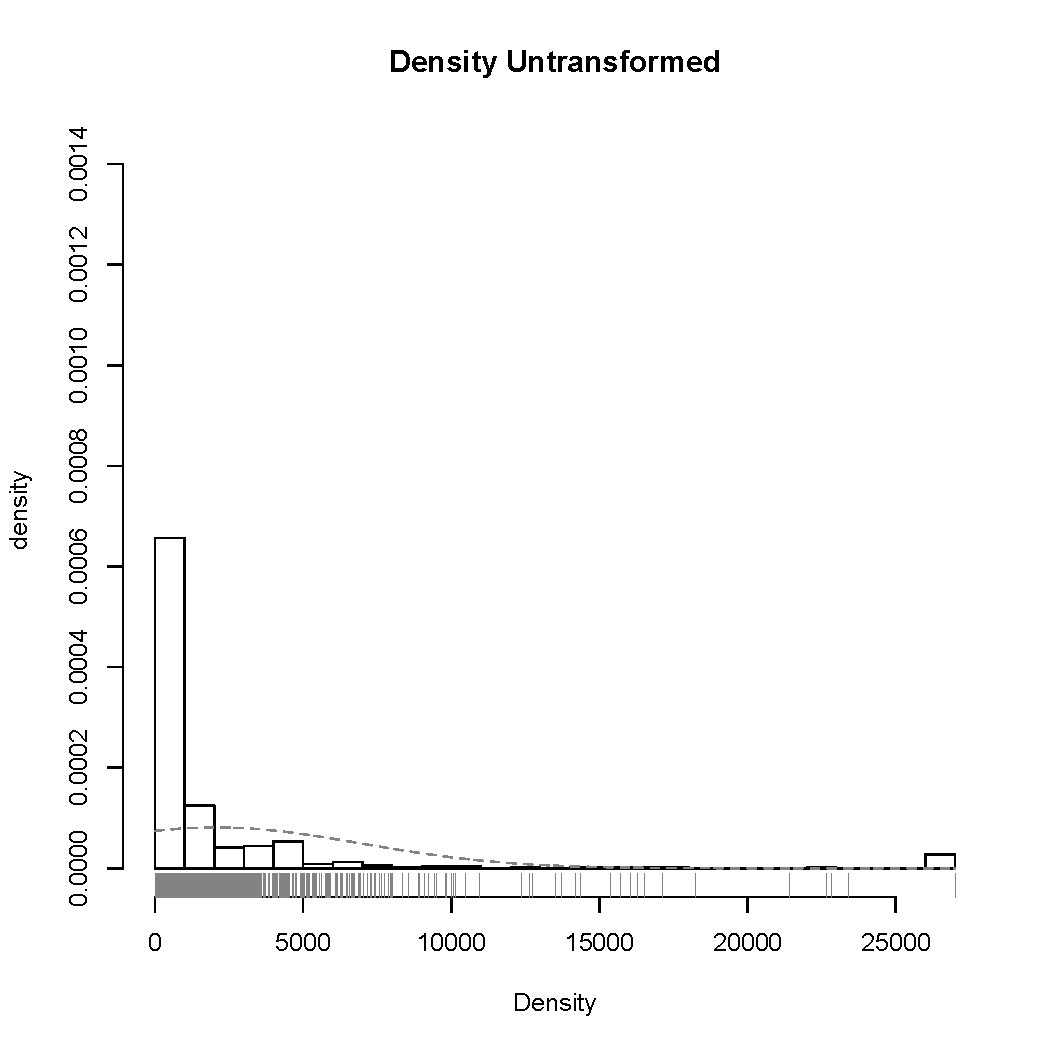
\includegraphics[scale=0.40]{Density.pdf}
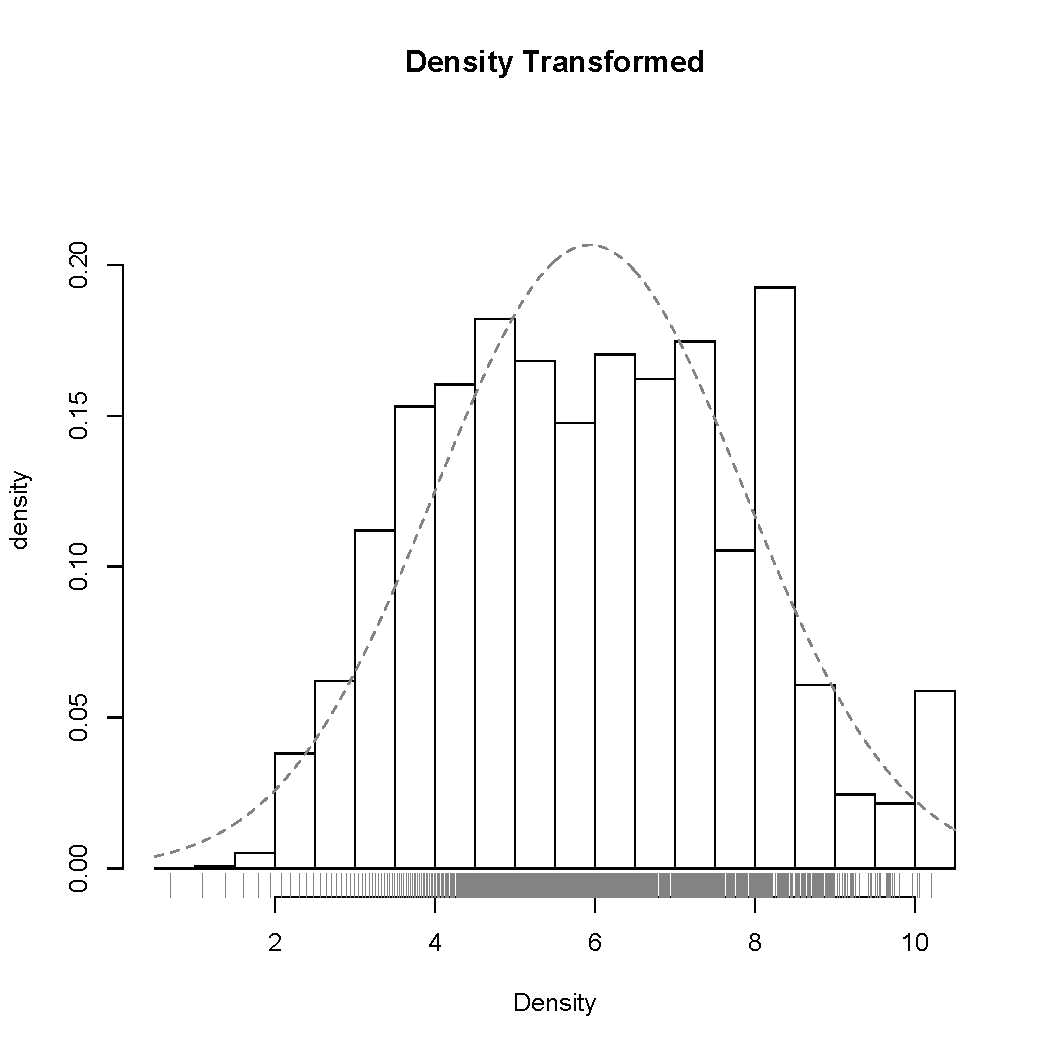
\includegraphics[scale=0.40]{logDensity.pdf}
\end{center}
\vspace{-0.2in}
\caption{Density variable: Left figure shows the fit when Gaussian distribution is imposed (CMW approach) to highly skewed data. Right figure shows the fit when log-normal assumption is applied (GCWM approach).}
\label{fig:vet1}
\end{figure}

The result of the transformation is a better AIC and BIC. \textcolor{red}{[Need a fuller sentence here.]} Table~\ref{comparingCWM_models} shows a considerable difference in BIC and AIC comparing CWM and GCWM. The five component CWM with a BIC of 285,268 is significantly higher than the four component GCWM with a considerably lower BIC of 89,568.
\begin{table}[!htbp] \centering
  \caption{Comparison of AIC and BIC for CWM versus GCWM models. \textcolor{red}{[Column~2 here is ``k''. What is ``k''?]}}\label{comparingCWM_models}
\begin{tabular}{@{\extracolsep{5pt}} rrrr}
\hline
Model & k & AIC & BIC \\
\hline
CWM & $1$ & $$$352,470$ & $$$352,661$ \\
& $2$ & $$$314,560$ & $$$314,949$ \\
& $3$ & $$$301,223$ & $$$301,812$ \\
& $4$ & $$$287,020$ & $$$287,808$ \\
& $\bm{5}$ &$$$\bm{284,283}$ & $$$\bm{285,268}$ \\
\hline
GCWM & $1$ & $$$111,129$ & $$$111,320$ \\
& $2$ & $$$90,039$ & $$$90,428$ \\
& $3$ & $$$89,476$ & $$$90,065$ \\
& $\bm{4}$ & $$$\bm{88,781}$ & $$$\bm{89,568}$ \\
& $5$ & $$$88,731$ & $$ $89,717$ \\
\hline
\end{tabular}
\end{table}

	We now investigate the results of GCWM in relation to the valuation of risk. For practical uses, finding clusters allows us to create different classifications of risk for various groups of drivers. \textcolor{red}{[The previous sentence seems to me to contain the key point. I think this should be highlighted in the introduction and, insofar as possible, expanded upon here and maybe in the conclusions.]} The following GCWM allows to cluster different drivers in groups allowing one to assign different rates to different clusters. \textcolor{red}{[What following GCWM?]}

After fitting the model, we then inspect the size of each cluster. The GCWM approach has chosen four components as the best model to represent the data. The size of each cluster is displayed in Table~\ref{table:sizeSev}. Attention is brought to largest quantity of drivers that are grouped into Cluster 4. This accounts for $ 46 \% $ of all drivers and is fairly concentrated in the center of Figure \ref{fig:vet1a}. From the results we can create an insurance model with the distinct characteristics.
\begin{table}[!htb]
\centering
\caption{Size of clusters for the GCWM a model.}
\label{table:sizeSev}
\begin{tabular}{rrrr}
\hline
Cluster 1   & Cluster 2  & Cluster 3   & Cluster 4    \\
\hline
1,683 & 5,766 & 848 & 7,093 \\
Red & Green & Blue & Teal \\
\hline
\end{tabular}
\end{table}
\begin{figure}[!htb]
\begin{center}
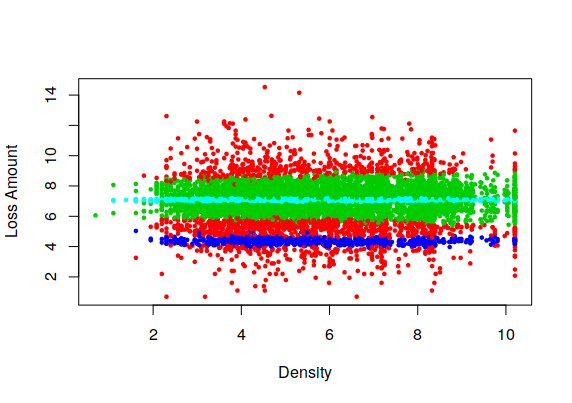
\includegraphics[scale=0.8]{SeverityPlot}
\end{center}
\vspace{-0.2in}
\caption{Showing clusters by color scheme: Cluster 1 - Red, Cluster 2 - Green, Cluster 3 - Blue, Cluster 4 - Teal for $LossAmount$ vs $Density$ on a log scale. \textcolor{red}{[The resolution of this figure could be higher. Similar for Figure~3.]}}
\label{fig:vet1a}
\end{figure}


The Cluster 3 drivers have both low variability and low average cost in claims, thus can be insured with a lower rate than other drivers. From a risk management perspective this is the most ideal case as these claims have very low variance and cost. Cluster 4 drivers have also low variability but a higher average cost, thus they would have a rate higher than Cluster 3. Cluster 2 drivers have the next highest cost and variability of the clusters, these drivers are colored in green in Figure \ref{fig:vet1}. The final cluster colored in red has the highest cost and variaiblity in claims out of any of the other clusters. From a risk management perspective this cluster would have the highest rate.


Table \ref{table:volSev} shows a breakdown of the types of drivers, ordered by volatility in descending order. Beginning with V1 volatility level, these drivers tend to have claims between $51$ to $154$, with a standard deviation of $13$, and a mean of $79$. That means that these drivers rarely exceed costs and tend to have very low volatility of claims. Moving onto V2 , these drivers have the second lowest level of volatility. Drivers in this range tend to have claims anywhere between $1,039$ to $1,324$, with a standard deviation of $52$, and a mean of $1,109$.  Proceeding to V3, \textcolor{red}{its} volatility in claims is greater than the preceding levels. Drivers in this cluster have claims anywhere between $221$ to $8841$, with a mean of $1,687$, and a standard deviation of $1284$. Finally, V4 denotes the level of highest volatility. Claims in this level  reach the highest recorded claim of $2,036,833$, a mean of $97,17$, and a standard deviation of $64,835$. \textcolor{red}{I think we should try to add monetary units; as a reviewer, this would annoy me.]}
%Table \ref{table:volSev} shows a breakdown of the types of drivers, ordered by volatility in descending order. Beginning with V1 volatility level, these drivers tend to have claims between \$51 to \$154, with a standard deviation of \$13, and a mean of \$79. That means that these drivers rarely exceed costs and tend to have very low volatility of claims. Moving onto V2 , these drivers have the second lowest level of volatility. Drivers in this range tend to have claims anywhere between \$1,039 to \$3,109, with a standard deviation of \$52, and a mean of \$3,109.  Proceeding to V3, it's volatility in claims is greater than the preceding levels. Drivers in this cluster have claims anywhere between \$221 to \$8841, with a mean of \$1,687, and a standard deviation of \$1284. Finally, V4 denotes the level of highest volatility. Claims in this level  reach the highest recorded claim of \$2,036,833, a mean of \$97,17, and a standard deviation of \$64,835.
% Paul: I do not know the monetary units of the prices, they are either in dollars or euros. 
\begin{table}[!htb]
\centering
\caption{Summarized volatility information of each cluster for Claims.}
\label{table:volSev}
\begin{tabular}{lrrrr}
\hline
Volatility Level (Cluster)     & Minimum & Mean  & Maximum & $\sigma$    \\
\hline
V1 (3) & 51  & 79 & 154 & \textbf{ 13} \\
V2 (4) & 1,039  & 1,109  &  1,324 & \textbf{ 52} \\
V3 (2) & 221 & 1,687  & 8,841  &\textbf{ 1,284}  \\
V4 (1) & 2 & 9,717 & 2,036,833  & \textbf{ 64,835}\\
\hline
\end{tabular}
\end{table}


Coefficients of clustered results are used to calculate premiums in car insurance. Table~\ref{severity_coef_table} (Appendix~\ref{app:tables}) shows the coefficients of the fitted model. In each cluster, statistical significance varies but overall the majority of coefficients are statistically significant.

In summary, the drivers have been clustered into four categories with distinct characteristics outlined in Table~\ref{table:volSev}. We have seen how using the results from GCWM, one can create an insurance model based on clustering algorithms with various levels of risk represented in each cluster. GCWM found a group that contains a clear majority of drivers, in which the volatility of their claims was extremely low regardless of $Density$ or $DriverAge$. The results show that GCWM may potentially find unique clusters that are otherwise hidden within the data.


 \subsubsection{Modeling Claims Frequency}

In this section, we model frequency of the French motor claims. We consider the covariates $Density$, $DriverAge$, $CarAge$,$Exposure$ and $Power$. The choice of covariates stems from the previously modelled single component ZIP \citep{Charpentier:2014}.
The GCWM is modelled with the linear formula
\begin{equation}
Claim Nb = Density + Exposure + Power \quad|\quad Exposure + Car Age,
\end{equation}
\textcolor{red}{[Same comment as before about the way this is presented.]}
where $Density$, $Exposure$, and $Power$ are explanitory variables in a Poisson model, while $Exposure$ and $Car Age$ are explantory for a Bernoulli model. As in Section 4.2.1, we also impose a log-normal assumption on the $Density$ covariate.
After fitting the model, GCWM has found two zero-inflated components and one Poisson component as the best model to represent the data. The size of each cluster is displayed in Table~\ref{table:sizeFreq} and we note a fairly even spread of the size across the three clusters.
\begin{table}[!htb]
\centering
\caption{Size of clusters for the GCWM a model. \textcolor{red}{[There is clearly something other than sizes in this table, i.e., the colours.]}}
\label{table:sizeFreq}
\begin{tabular}{rrrr}
\hline
Cluster 1   & Cluster 2  & Cluster 3   \\
100492 & 163503 & 149174 \\
Red & Green & Blue  \\
\hline
\end{tabular}
\end{table}

Similarly to modelling severity, the GCWM finds clusters with unique characateristics. This is evident when looking at the Claims vs. Density plot (Figure~\ref{frequencyGraph}). We see that the GCWM has split up the drivers into three groups based on the Density of cities. Table \ref{summarycovariates} shows that Cluster 2 drivers live in the least dense cities with a mean of 7.86 km on the log-scale. Followed by Clusters 3 and 1 with a mean of 5.23 km and 3.38 km, respectively.
\begin{figure}[!ht]
\begin{center}
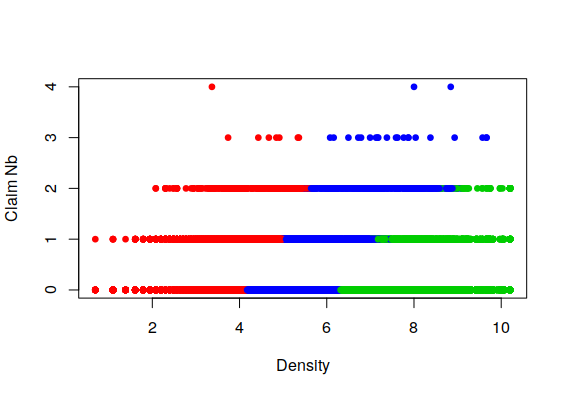
\includegraphics[scale=0.80]{frequency.png}
\end{center}
\vspace{-0.2in}\caption{Showing clusters in color for Frequency vs Density under log-normal assumptions.}
\label{frequencyGraph}
\end{figure}
\begin{table}[!htb]
 \begin{center}
 \caption{Summary of each cluster with log-normal assumptions for the $Density$ covariate measured in km on a log scale.} \label{summarycovariates}
\begin{tabular}{lrrrrr}
\hline
Cluster  & Color & Minimum & Mean & Maximum & $\sigma$  \\
\hline
1 &   Red         & 0.69    & 3.38 & 5.60    & 0.60  \\
2 &  Green       & 6.29    & 7.86 & 10.20   & 1.03  \\
3 &  Blue        & 4.13    & 5.23 & 9.66    & 0.65 \\
\hline
\end{tabular}
\end{center}
\end{table}

Table \ref{frequencySummary} (Appendix~\ref{app:tables}) shows a summary of the coefficients for the zero-inflated model. The
significance codes are the same as for Table \ref{severity_coef_table}. In each cluster we can see that the majority of the coefficients are significant, particularly in the zero-count model for the Bernoulli. Cluster~1 was selected to be strictly a Poisson model by the likelihood ratio test defined in \eqref{LRTest}. \textcolor{red}{[Reword previous sentence.]} In summary, we see that the GCWM can account for zero-inflated data in pricing.


\section{Simulation Study}\label{sec:sim}

Two simulation studies are conducted to determine the validity of the log-normal assumption and the effectiveness of the Bernoulli-Poisson partitioning method. The first section outlines the need for a non-Gaussian assumption for the covariates. The second section shows the classification accuracy and other relevant analysis for the Bernoulli-Poisson method.


\subsection{Simulation Study for GCWM}


In this section, we show how the proposed methodology works for different simulation settings. The simulation study was generated based on the regression coefficients of the CASdataset used in the previous section. The aim of the simulation study is to test the accuracy and ability of both GCWM a and CWM to return estimates of true parameters when one or more of the covariates is log-normal and the other two are Gaussian. This was designed to test both functions in the event when one of the covariates is non-Gaussian. The motivation behind this is fact is that many covariates used in insurance are likely to come from non-Gaussian distributions. Thus this was aimed to test the relevancy of CWM, which treats all covariates as Gaussian.

We define Model 1 as the baseline model in which the coefficients were generated for \textbf{CASdataset} and reported in upper portion of Table 2. \textcolor{red}{[Some problems with the previous sentence: (1) I think we mean ``Model~1 is the baseline model, where the coefficients\ldots''; (2) I don't fully understand the reference to Table~2; and (3) Table~2, as with all other tables and figures, should be referenced in \LaTeX\ via a nickname. I won't repeat the latter comment but please make sure all tables and figures are referenced using nicknames.]} These coefficients were then rounded and treated as true parameters. \textcolor{red}{[Why rounded?]} A simulation with three GLM mixture components was then generated around these true parameters in which the third covariate $X_3$ was log-normal. Stemming from this, both CWM and  GCWM are run. The  GCWM a treats $X_3$ as a log-normal covariate. \textcolor{red}{[Please read the last three sentences carefully.]}

\textcolor{red}{[Do not use past tense anywhere but the conclusions section. I have made some edits but I am sure I missed some others.]} The results for Model 1 are summarized in upper portion of Table 3 based on the performance of the  GCWM a approach. The simulation is run $1000$ times. We report the percentage of runs for each predictor and the corresponding intercept in each mixture component under the assumption of $5\%$ error. For example, predictor $X_2$ in the component 2 of Model 1 reports $90.10\%$ accuracy. \textcolor{red}{[How does a predictor report?]} This means that $90.1\%$ of the time the true parameter is estimated within $5\%$ error. In this setting, predictor $X_1$ in the second component is insignificant in the real data set. The purpose of including this parameter in Model~1 is to test the sensitivity of  GCWM a for insignificant predictors. In this case, the result of zero is underlined and means that it \textcolor{red}{[what?]} has no influence on the response variable in this simulation. Further, we create Models 2, 3, 4 and 5 by altering the parameters of Model~1 by $+30\%$, $-30\%$, $+50\%$, and $-50\%$, respectively, and keeping the second covariate of the second component as an insignificant predictor form the CASdataset model. This is done to test the accuracy of  GCWM \textcolor{red}{a} to the  sensitivity of coefficients. Based on the results in Table \ref{gcwmAccuracy}, we can see that GCWM performs well for all simulation settings.
\begin{table}[!htb]
\centering
\caption{GCWM a vs CWM Accuracy: covariate $X_3$ is treated as log-normally distributed, while the rest of covariates are of the Gaussian type.}
\label{gcwmAccuracy}
\begin{tabular}{ll|rrrr|rrrrr}
\hline
Mod. & $G$ & Int. & $X_1$ &$X_2$ & $X_3$& Int. & $X_1$ &$X_2$ & $X_3$  \\
\hline
1     & 1         & 93.00\%   & 90.10\%  & 93.00\%  & 93.10\% & 0.00\% & 0.00\% & 0.00\% & 0.00\%   \\
      & 2         & 90.10\%   & \underline{0.00\%}   & 90.10\%  & 90.10\% & 0.00\% & 0.00\% & 0.00\% & 0.00\%  \\
      & 3         & 99.20\%   & 99.10\%  & 99.20\%  & 99.20\% & 0.00\% & 0.00\% & 0.00\% & 0.00\%  \\
      \hline
2     & 1         & 89.80\%   & 89.20\%  & 89.80\%  & 89.80\% & 0.00\% & 0.00\% & 4.60\% & 0.00\%  \\
      & 2         & 89.20\%   &\underline{0.00\%}   & 89.20\%  & 89.20\% & 0.00\% & \underline{0.00\%} & 0.00\% & 0.00\%   \\
      & 3         & 99.20\%   & 99.20\%  & 99.20\%  & 99.20\% & 0.00\% & 0.20\% & 1.70\% & 0.00\%  \\
      \hline
3     & 1         & 100.00\%  & 100.00\% & 100.00\% & 100.00\%  & 0.00\% & 0.00\% & 0.00\% & 0.00\% \\
      & 2         & 100.00\%  & \underline{0.00\%}   & 100.00\% & 100.00\% & 0.00\% & 0.00\% & 0.00\% & 0.00\% \\
      & 3         & 99.20\%   & 99.20\%  & 99.20\%  & 99.20\%  & 0.00\% & 0.00\% & 0.00\% & 0.00\%\\
      \hline
      4 & 1 & 88.60\% & 86.80\% & 88.60\% & 87.00\%  & 0.00\% & 0.00\% & 0.00\%  & 0.00\%  \\
  & 2 & 86.90\% &\underline{ 0.00\%}  & 86.90\% & 86.90\% & 0.00\% & \underline{0.00\%} & 0.00\%  & 0.00\%  \\
  & 3 & 99.20\% & 99.20\% & 99.20\% & 99.20\% & 0.00\% & 0.00\% & 0.00\%  & 0.00\% \\
      \hline
5 & 1 & 85.90\% & 84.90\% & 85.60\% & 85.90\% & 0.00\% & 0.00\% & 0.00\%  & 0.00\% \\
  & 2 & 85.00\% &\underline{ 0.00\%}  & 84.90\% & 84.90\% & 0.00\% & \underline{0.00\%} & 0.00\%  & 0.00\%  \\
  & 3 & 99.20\% & 99.20\% & 99.20\% & 99.20\% & 0.00\% & 0.20\% & 10.90\% & 0.00\% \\
      \hline
\end{tabular}
\end{table}

% Table 4 provides the summary of the results when CWM was used in the analysis of the same models considered in Table 3. Commented sentanced 
In line with expectations we note that barely any of the simulation runs are estimated correctlly, as most of the results are zero. This means that the performance of CWM approach is poor in presence of one non-Gaussian covariate which in this case is a log-normal covariate. 

Table \ref{mseTable} provides the summary of mean squared errors\footnote{The MSE is computed using the following formula MSE $(\beta) = \frac{\sum_i^n (\beta_i - \hat\beta_i ) ^2}{n}$. Here, $n$ accounts for the number of simulation runs, $\beta$ is the true parameter of interest while $\hat{\beta}$ accounts for its estimate.} (MSEs) of each parameter of the models for the same simulated runs in Table~\ref{gcwmAccuracy}. \textcolor{red}{[Try to avoid footnotes.]} The MSEs related to the predictor variables for all models and their corresponding components are about zero indicating that  GCWM a approach performs well. This is also a result of having a small size coefficients.
\begin{table}[h!]
\centering
\caption{ GCWM results: the summary of MSE for all parameters used in five models. The covariate $X_3$ is treated as log-normal distributed, while the rest of covariates are Gaussian. These results correspond to same simulated runs as those in Table~\ref{gcwmAccuracy}.}
\label{mseTable}
\begin{tabular}{ll|rrrrrrrr}
\hline
Mod. & $G$ & $\beta_o$ &  MSE($\beta_o$)   &  $\beta_1$ & MSE($\beta_1$)& $\beta_2$ &MSE($\beta_2$)   & $\beta_3$ &  MSE($\beta_3$)  \\
\hline
1     & 1         & 1028& (11.353)   & 0.03& (0.00)  & 3.5& (0.00)    & -380& (0.09)   \\
      & 2         & 1600& (0.000)     & -0.01&(0.00) & 1.5&(0.00)    & -250&(0.00)   \\
      & 3         & 40000&(0.035)    & -6.00&(0.00) & -305&(0.00) & 1100&(0.47)   \\
\hline
2     & 1         & 1350&(0.167)     & 0.04&(0.00)  & 4.5&(0.00)    & -500&(0.03)   \\
      & 2         & 2080& (0.001)     & 0.04&(0.00)  & 2.0&(0.00)    & -325&(0.00)   \\
      & 3         & 52000& (0.012)    & -8.00&(0.00) & 450&(0.00)  & 14300&(0.01)  \\
\hline
3     & 1         & 720& (0.001)      & 0.02&(0.00)  & 2.5&(0.00)   & -266&(0.00)   \\
      & 2         & 1100& (0.008)     & 0.00&(0.00)  & 1.1&(0.00)    & -17511&(0.00) \\
      & 3         & 28000& (0.002)    & -4.20&(0.00) & 245&(0.00)  & 7700.&(0.00) \\
\hline
4     & 1         & 1650&(13.056)   & 0.05&(0.00)  & 5.3&(0.00)    & -570&(0.00)   \\
      & 2         & 2400& (0.000)     & -0.01&(0.00) & 2.3&(0.00)    & -375&(0.00)   \\
      & 3         & 60000& (0.051)    & -9.00&(0.00) & -457&(0.00) & 16500&(0.00)  \\
\hline
5     & 1         & 500& (1.115)     & 0.02&(0.00)  & 2.0&(0.00)    & -190&(0.05)   \\
      & 2         & 800& (0.003)      & 0.00&(0.00)  & 0.8&(0.00)    & -120&(0.00)   \\
      & 3         & 20000& (0.000)    & -3.00&(0.00) & -150&(0.00) & 5500&(0.00)  \\
      \hline
\end{tabular}
\end{table}
\begin{table}[!htb]
\centering
\caption{CWM results: the summary of MSE for all parameters used in five models. All three covariates are treated as Gaussian. These results correspond to same simulated runs as those in Table~\ref{gcwmAccuracy}.}
\label{my-label}
\begin{tabular}{ll|rrrrrrrr}
\hline
Mod. & $G$ & $\beta_o$ &  MSE($\beta_o$)   &  $\beta_1$ & MSE($\beta_1$)& $\beta_2$ &MSE($\beta_2$)   & $\beta_3$ &  MSE($\beta_3$)  \\
\hline
1     & 1         & 1028& ($\cdot$)   & 0.03&  ($\cdot$)   & 3.5&  ($\cdot$)    & -380&  ($\cdot$)    \\
      & 2         & 1600&  ($\cdot$)      & -0.01& ($\cdot$)  & 1.5& ($\cdot$)     & -250& ($\cdot$)  \\
      & 3         & 40000& ($\cdot$)     & -6.00& ($\cdot$)  & -305& ($\cdot$)  & 1100& ($\cdot$)    \\
\hline
2     & 1         & 1350& ($\cdot$)     & 0.04& ($\cdot$) & 4.5& ($\cdot$)    & -500& ($\cdot$)  \\
      & 2         & 2080&  ($\cdot$)    & 0.04& ($\cdot$)   & 2.0& ($\cdot$)     & -325& ($\cdot$)   \\
      & 3         & 52000&  ($\cdot$)     & -8.00& (0.006)  & 450& (44.1)   & 14300& ($\cdot$)  \\
\hline
3     & 1         & 720&  ($\cdot$)     & 0.02& ($\cdot$)   & 2.5& ($\cdot$)    & -266& ($\cdot$)    \\
      & 2         & 1100&  (65.814)     & 0.00& ($\cdot$)   & 1.1& ($\cdot$)     & -17511& ($\cdot$)  \\
      & 3         & 28000& ($\cdot$)   & -4.20& ($\cdot$)  & 245& ($\cdot$)   & 7700.& ($\cdot$)  \\
\hline
4     & 1         & 1650& ($\cdot$)    & 0.05& ($\cdot$)  & 5.3& ($\cdot$)    & -570& ($\cdot$)  \\
      & 2         & 2400&  ($\cdot$)     & -0.01& ($\cdot$)  & 2.3& ($\cdot$)    & -375& ($\cdot$)    \\
      & 3         & 60000&  ($\cdot$)     & -9.00& ($\cdot$)  & -457& ($\cdot$)  & 16500& ($\cdot$)   \\
\hline
5     & 1         & 500&  ($\cdot$)     & 0.02& ($\cdot$)   & 2.0& ($\cdot$)   & -190& ($\cdot$)  \\
      & 2         & 800&  ($\cdot$)      & 0.00& ($\cdot$)   & 0.8& ($\cdot$)    & -120& ($\cdot$)  \\
      & 3         & 20000&  ($\cdot$)     & -3.00& (0.003)  & -150& (4.7) & 5500& ($\cdot$) \\
\hline
\end{tabular}
\end{table}



In contrary to the results reported in Table 5, these results in Table 6 are significantly different. We can observe that the MSEs for most of the models and their corresponding coefficients are not calculated at all due to convergence failures and as such they are shown as $(\cdot)$. This is not surprising because Table 4 shows the accuracy of CWM is not good when attempting to model non-Gaussian predictors as Gaussian. \textcolor{red}{[Why are we talking about Tables 4, 5 and 6 here? Again, nicknames should be used.]}

In summary, our simulation results showed good performance of the GCWM approach in modeling non-Gaussian covariates. More specifically, these results show high accuracy when covariates are log-normal. In contrary, CWM fails to estimate parameters accurately when the Gaussian assumption is violated.

\clearpage\textcolor{red}{[I have stopped here. Please make similar edits I have suggested thus far to the remainder of the paper.]}


\subsection{Simulation Study - Bernoulli-Poisson Partitioning}

In this section we show how the Bernoulli-Poisson (BP) partitioning method behaves under different conditions. The components were genereated under similar coefficients taken from the \textbf{CASDatasets} package. The coefficients were rounded and treated as true parameters to which data was generated from. The mean and standard deviation of the covariates within each component was also taken into account when generating data. The first simulation examines the performance of the GCWM model for classification. We generate three components each with sample size $N=1000$ for a total of $3000$ simulated points.
The model generated is similar to the mean and standard deviations of Table \ref{summarycovariates}. Consider three simulated covariates and 
\begin{equation}
SimClaimsNb = SimDriverAge + SimDensity + SimCarAge 
\end{equation}
as the GLM. The covariates $SimDriverAge$, $SimDensity$, and $SimCarAge$ are considered for both the Poisson and Bernoulli models. 
 Here the GCWM is fitted to the simulated data and used to classify into three components. The misclassification rate is calculated by the proportion of true labels placed in other components by the GCWM a model.  The results of the simulation is based on the generated dataset are presented in Table \ref{misclassTable}. The total misclassification rate  is $1.8 \% $ and the majority of misclassified components are between components two and three.
\begin{table}[!htb]
\begin{center}
\caption{Misclassfication rate and label comparison of generated data.}
\label{misclassTable}
\begin{tabular}{r r r r r r}
\hline\hline
    True Labels       &  \multicolumn{3}{r}{ Classified }   & Misclassification Rate  &  \\ \cmidrule{2-4}
   & 1                              & 2   & 3   &                            &  \\ \hline
1              & 992                            & 3   & 5   & 0.80 \%                                      &  \\
2              & 0                              & 990 & 10  & 1.00 \%                                       &  \\
3              & 15                             & 20  & 965 & 3.50 \%                                      &  \\  \hline
                \multicolumn{4}{r}{Overall Misclassification Rate}        & 1.80 \%                  & \\
        		\multicolumn{4}{r}{Average Purity} & 98.23 \%  
        		\\ \hline
                \multicolumn{4}{r}{Adjusted Rand Index} & 0.9479 &  \\
    \hline\hline
\end{tabular}
\end{center}
\end{table}

The experiment is expanded further to show how Bernoulli-Poisson partitioning behaves over 1000 runs and under two different conditions. The first condition is defined as follows. The mean and standard deviations are taken as given by the estimated  ZIP components from the \textbf{CASDataset}. The second condition involves adjusting the means of two of the covariates so they are closer to each other. The goal is to show that the BP-method holds its use even when means among covariates are close. The conditions are divided into two scenarios. In the first scenario which we consider ``normal", the covariate means are taken directly from the sample data. In the second scenario ``close" as the covariate means are manipulated so that they are closer to each other within some degree. This is a common problem in classification where if the means among two different components are close, then misclassification rate increases \citep{LimHwa}. Experiment 2 tests the accuracy of 3 different partitioning methods to initialize a zero-inflated model. The Poisson partitioning method assumes that the presence of non-zeros will provide a better partitioning of the data-set. The Bernoulli partitioning method assumes that the presence of excess zeros will determine the best partitioning of the data-set. Finally the BP partitioning method assumes that both methods are weighed equally and therefore both must be taken into account when partitioning the dataset. The mean and standard deviation of each measurement is provided in Table \ref{table:exper2}.

\begin{table}[!htb]
\begin{center}
\caption{Experiment 2: mean and standard deviations for each statistic compared across methods.}
\label{table:exper2}
\begin{tabular}{rrrrrrrr}
\hline\hline
Type   & Condition & Poisson & ($\sigma $) & Bernoulli & ($ \sigma $) & BP & ($ \sigma $) \\
\hline
Misclassification Rate& normal        & 1.70\% & (6.00)       & 1.60\%  & (6.00)         & 1.10\% & (0.02)         \\
       & close      & 5.00\% & (7.00)       & 6.00\% & (2.00)         & 7.00\% & (4.00)         \\
Average Purity & normal     & 98.87\% & (2.00)    & 98.91\% & (2.25)      & 99.18\% & (0.81)     \\
       & close       & 95.38\% & (4.00)    & 94.55\% & (1.00)      & 96.95\% & (0.48)      \\
Adjusted Rand Index  & normal      & 0.9662 & (0.07)    & 0.9677  & ( 0.07)     & 0.9729 & (0.0217)      \\
       & close         & 0.8706 & (0.08)    & 0.8366 & (0.04)      & 0.8538 & ( 0.0453) \\
       \hline\hline
\end{tabular}
\end{center}
\end{table}
Several findings are concluded from Table \ref{table:exper2}. Under condition normal, the BP method shows better performance in error and is found to be less sensitive than other methods with an error rate of $ 1.10 \% $ and a standard deviation of $ 0.02 \% $.  Further findings show that when close condition is imposed then Bernoulli has better performance in terms of accuracy. The Adjusted Rand Index\footnote{Having $n_{ij}$ to be a matrix entry, $a_i$ to be the $i$th row sum, and $b_j$ to be the $j$th column sum  from the classification matrix of Table \ref{misclassTable}, the Adjusted Rand Index is calculated as  $ARI = \frac{ \sum_{ij} \binom{n_{ij}}{2} - [\sum_i \binom{a_i}{2} \sum_j \binom{b_j}{2}] / \binom{n}{2} }{ \frac{1}{2} [\sum_i \binom{a_i}{2} + \sum_j \binom{b_j}{2}] - [\sum_i \binom{a_i}{2} \sum_j \binom{b_j}{2}] / \binom{n}{2} }$. } (ARI) shows good measurements overall, but in particular the BP partitioning method under normal scenario has a very good ARI with a small standard deviation. The Average Purity \footnote{ The Average Purtiy is calculated as $AP = \frac{1}{N} \sum_i  n_{i i}.$} (AP) of the BP partitioning method is the best out of all other methods, which is relevant to estimating coefficients accurately for optimization.

\section{Conclusion}

In this paper, we extend the class of generalized linear mixture CWM models by accomplishing two main goals. First, we proposed the methodology that allows for continuous covariates to follow a non-Gaussian distribution. Imposing Gaussian distribution on a skewed data may result in an suboptimal model fit. Second, we proposed a new Poisson CWM methodology that uses Bernoulli-Poisson partitioning method and allows for implementation of zero-inflated Poisson CWM model (ZI-GCWM). We name our proposed model class as the Generelized Cluster-Weighted Model (GCWM), to reflect the two extensions made to the existing CWM class of models.

Our proposed GCWM models allow for great applications in predictive modeling of insurance claims by overcoming a few limitations of the current CWM models. The ZI-GCWM allows for finding clusters within claims frequency which is an important information in risk classification and modeling of claims frequency. Further, some insurance rating variables used in the predictive modeling of severity claims may not strictly follow Gaussian assumptions, for example driver's age or car age, when treated as continuous covariates. An adequate extension to non-Gaussian covariates can be considered to relax current assumptions and improve the model fit. Given our data, we convincingly demonstrated that there is a need for a log-normal assumption in the $Density$ covariate, and by making it we have consideredly the model fit. 

The results of our extensive simulation study showed the excellent performance of the proposed models in case of modeling non-Gaussian covariates. We found  that current CWM model fails to estimate the parameters accurately when the Gaussian assumption is violated. The GCWM a shows significant improvement in the model fit over the CWM model based on AIC and BIC criteria. We also tested Bernoulli-Poisson partitioning of zero-inflated GCWM under different conditions and found that our proposed partitioning method has a very low misclassification rate, high average purity, and high average rand index.

Our approach is relevant to the actuarial pricing and risk management when current practices are based on implementation of various GLM models. Further extension of this work may incorporate modifications of the CWM family to allow for modeling limited depended variable or the right-censored data structure (refer to \cite{miljkovic2015} and \cite{miljkovic+orr:2017}).



\appendix
\section{Derivation of the Log-normal Distribution }
Consider a random variable $U$ having univariate log-normal distribution with parameters $\mu \in \mathbb{R}$ and $\sigma \in \mathbb{R}_+ $. Have $u \in \mathbb{R}_+$, then the probability density function of random variable $U$ is defined as \footnote{For full definition see \cite{johnson1995continuous}}
$$\mathcal{LN}(u; \mu, \sigma) = \frac{1}{u\sigma\sqrt{2\pi}}\exp\left[-\frac{(\ln u - \mu)^2}{2\sigma^2}	\right].$$
\text{Further, if random variable }$X$\text{ is normally distributed i.e. }$ X \sim \mathcal{N}(x; \mu, \sigma) $, then $U := \exp{(X)}\sim \mathcal{LN}(u; \mu, \sigma) $.
To see this, let $p_U(u)$, and $ p_X(x) $ be the probability density functions of $U$ and $X$ respectively. By the change of variables theorem (see \cite{murphy2012machine} section 2.6.2.1) the density $p_U(u)$ is derived as
$$p_U(u) = p_X(\ln u )\frac{\partial}{\partial u} \ln u  =  p_X(\ln u ) \frac{1}{u} =  \frac{1}{u\sigma\sqrt{2\pi}}\exp\left[-\frac{(\ln u - \mu)^2}{2\sigma^2}	\right].$$\newline
 We extend to a log-normal multivariate case where the random variable $\bm{U} $ is parameterized by $ \bm{\mu} \in \mathbb{R}^p$ and $\bm{\Sigma} \in  \mathbb{R}_{+}^{p \times p} \label{changeVarUni} $.
\begin{lemma}
Let the random variable $\bm{X}$ have multivariate normal distribution ie. $\bm{X} \sim \mathcal{MVN}(\bm{x}, \bm{\mu},\bm{\Sigma}) $, then $\bm{U} := \exp(\bm{X} ) \sim  f^U(\bm{u}; \bm{\mu } , \bm{\Sigma} )$. Here
have $\bm{u} \in \mathbb{R}_{+}^p $ and the probability density function $f^U$ is
$$ f^U(\bm{u}; \bm{\mu } , \bm{\Sigma} )= \frac{1}{(\prod_{i=1}^{p}u_{i})| \bm{\Sigma} |(2 \pi)^{\frac{p}{2}}}   \exp\left[-\frac{1}{2}(\ln \bm{u} -\bm{\mu})^{'}  \bm{\Sigma}^{-1}(\ln \bm{u} -\bm{\mu})\right].  $$
\end{lemma}
\begin{proof}
Let $f^U(\bm{u}; \bm{\mu},\bm{\Sigma})$ and $f^X(\bm{x}; \bm{\mu},\bm{\Sigma})$ be the probability density functions of $\bm{U}$ and $\bm{X}$ respectively. By the multivariate change of variables theorem (see \cite{murphy2012machine} section 2.6.2.1), we derive the log-normal distribution, where $ | \det J_{\ln} (u) | $ is the absolute value of the determinant for the Jacobian of the multivariate transformation $\ln(\bm{U}) = \bm{X} $. Hence,
\begin{align*}
 | \det J_{\ln} (\bm{u}) | & = \prod_{i=1}^p u_i^{-1}, \; \text{and} \; \\
   f^U(\bm{u}; \bm{\mu},\bm{\Sigma})  & =  f^X(\ln \bm{u}; \bm{\mu},\bm{\Sigma})  | \det J_{\ln} (u) | \\
  & = f^X(\ln \bm{u}; \bm{\mu},\bm{\Sigma})\prod_{i=1}^p u_i^{-1} \\
  & =  \frac{1}{(\prod_{i=1}^{p}u_{i})| \bm{\Sigma} |(2 \pi)^{\frac{p}{2}}}   \exp\left[-\frac{1}{2}(\ln \bm{u} -\bm{\mu})^{'}  \bm{\Sigma}^{-1}(\ln \bm{u} -\bm{\mu})\right].
  \end{align*}
\end{proof}

\section{Tables}\label{app:tables}

\begin{center}
\begin{sidewaystable}
\caption{ Summary of coefficients for severity clusters.}
\label{severity_coef_table}
\begin{tabular}{|l|rrc|rrc|rrc|rrc|}
\hline\hline
         & V1         & (Red)     &    & V2         & (Green)   &    & V3          & (Blue)     &    & V4          & (Teal)     &    \\
Coefficient \footnote{The significance codes are defined as $  P < 0.001 : $  (***), $0.001 < P < 0.01:$ (**), $  0.01 < P < 0.05:$ (*),\\ $0.05 < P < 0.10 : $ (.) %Nik: something wrong here; all of these could be considered $\approx 0$... use < some value. \\
pertaining to the $P$ value of the specific coefficient.}      & Estimate   & Error     & P   & Estimate   & Error     & P   & Estimate    & Error      & P   & Estimate    & Error      & P   \\ \hline
Intercept & 7.876  & 0.137 & *** & 7.180  & 0.061 & *** & 4.673   & 0.014 & *** & 7.077  & 0.003 & *** \\
Density   & -0.031 & 0.009 & *** & 0.005  & 0.004 &     & -0.011 & 0.001 & *** & 0.002  & 0.002 &     \\
C2        & -0.172 & 0.080 & *   & 0.064  & 0.034 & .   & 0.020 & 0.001 & **  & 0.008  & 0.002 & *** \\
C3        & -0.396 & 0.080 & *** & 0.108  & 0.034 & **  & 0.010  & 0.007 &     & 0.003  & 0.002 & .   \\
C4        & -0.642 & 0.081 & *** & -0.033 & 0.035 &     & 0.034  & 0.007 & *** & 0.005  & 0.002 & **  \\
C5        & -0.500 & 0.090 & *** & 0.066 & 0.039 & .   & 0.069  & 0.007 & *** & 0.011  & 0.002 & *** \\
D2        & -0.535 & 0.083 & *** & -0.168 & 0.038 & *** & -0.217 & 0.009 & *** & -0.006 & 0.001 & *** \\
D3        & -0.607  & 0.084 & *** & -0.241 & 0.038 & *** & -0.205 & 0.009 & *** & -0.008 & 0.001 & *** \\
D4        & -0.390 & 0.099 & *** & -0.122 & 0.045 & **  & -0.200 & 0.0106 & *** & -0.009  & 0.002 & *** \\
D5        & 0.123 & 0.101 &     & 0.035  & 0.047 &     & -0.138 & 0.010 & *** & -0.002 & 0.002 &     \\
R23       & 0.003 & 0.131  &     & -0.016 & 0.053 &     & -0.001 & 0.012 &     & 0.002  & 0.006 &     \\
R24       & -0.232 & 0.054 & *** & -0.017 & 0.023 &     & -0.102 & 0.005 & *** & -0.015 & 0.013 & *** \\
R25       & 0.144  & 0.096 &     & -0.184 & 0.043 & *** & -0.065 & 0.009 & *** & -0.016 & 0.024 & *** \\
R31       & -0.009 & 0.073 &     & 0.055  & 0.031 & .   & -0.141 & 0.008 & *** & -0.003 & 0.018 & .   \\
R52       & -0.303 & 0.064 & *** & 0.012   & 0.028 &     & -0.142 & 0.006  & *** & -0.015 & 0.038 & *** \\
F53       & -0.153 & 0.063 & *   & 0.095  & 0.028 & *** & -0.012 & 0.006  & *   & -0.014 & 0.001 & *** \\
R54       & -0.222 & 0.082 & **  & 0.074  & 0.037 & *   & -0.122 & 0.007 & *** & -0.015  & 0.002 & *** \\
R72       & -0.098 & 0.072 &     & 0.175  & 0.031 & *** & -0.081 & 0.007 & *** & -0.007 & 0.002 & *** \\
R74       & -0.236 & 0.142 & .   & -0.114 & 0.067 & .   & 0.466  & 0.016 & *** & -0.019 & 0.003 & *** \\
P-FGH     & 0.123 & 0.033 & *** & 0.012 & 0.015 &     & 0.001    & 0.003 &     & 0.002  & 0.001 & *   \\
P-Other   & 0.131  & 0.045 & **  & 0.075   & 0.020 & *** & 0.012  & 0.003 & **  & 0.005  & 0.001  & *** \\
GR        & -0.095 & 0.031 & **  & -0.029 & 0.014 & *   & 0.005   & 0.002 & .   & -0.005 & 0.001 & *** \\
\hline\hline
\end{tabular}
\end{sidewaystable}

\begin{sidewaystable}
\caption{Summary of coefficients for frequency clusters.}
\label{frequencySummary}
\begin{tabular}{|l|rrc|rrc|rrc|}
\hline\hline
          & Cluster 1 & (Red) &   & Cluster 2 & (Green) &  & Cluster 3 & (Blue) &   \\
Coefficient \footnote{The significance codes are defined as $  P < 0.001 : $  (***), $0.001 < P < 0.01:$ (**), $  0.01 < P < 0.05:$ (*),\\ $0.05 < P < 0.10 : $ (.) %Nik: something wrong here; all of these could be considered $\approx 0$... use < some value. \\
pertaining to the $P$ value of the specific coefficient.}             & Estimate  & Error & P   & Estimate  & Error   & P   & Estimate  & Error  & P  \\
 \hline
(Intercept) & -10.199   & 0.109 & *** & -7.217    & 0.216   & *** & -13.694   & 0.099  & *** \\
Density     & 1.860     & 0.027 & *** & 0.442     & 0.013   & *** & 1.771     & 0.013  & *** \\
Exposure    & 0.825     & 0.040 & *** & 0.726     & 0.192   & *** & 0.745     & 0.046  & *** \\
P-GH        & -0.063    & 0.030 & *   & -0.004    & 0.035   &     & 0.013     & 0.030  &     \\
P-Other     & -0.019    & 0.042 &     & 0.049     & 0.043   &     & 0.107     & 0.040  & **  \\
\hline
(Intercept) &          &      &    & 2.424     & 0.188   & *** & 1.886     & 0.356  & *** \\
Exposure    &          &      &    & -5.871    & 0.758   & *** & 16.520    & 2.990  & *** \\
C2          &          &      &    & -0.541    & 0.176   & **  & -0.922    & 0.368  & *   \\
C3          &          &      &    & -1.217    & 0.201   & *** & -2.263    & 0.553  & *** \\
C4          &          &      &    & -1.265    & 0.225   & *** & 10.805    & 72.677 &     \\
C5          &          &      &    & -0.808    & 0.266   & **  & -6.355    & 30.867 &   \\
\hline\hline
\end{tabular}
\end{sidewaystable}
\end{center}

\bibliographystyle{elsart-harv}
\bibliography{GLM_Mixtures_2018}

\end{document}


